% In this file you should put the actual content of the blueprint.
% It will be used both by the web and the print version.
% It should *not* include the \begin{document}
%
% If you want to split the blueprint content into several files then
% the current file can be a simple sequence of \input. Otherwise It
% can start with a \section or \chapter for instance.

\section{Introduction and the main result}
In this article, we study the transition matrix between two famous bases,
the Specht basis and the \( \SL_2 \)-web basis, for the irreducible representation
of the symmetric group \( \SYM_{2n} \) indexed by the partition \( (n,n) \).
Motivated by Rhoades's work~\cite{Rho19}, we give a combinatorial interpretation
for entries of the transition matrix as a certain class of permutations,
and present their interesting properties.

For an integer \( n\ge 1 \), let \( \SYM_{2n} \) be the symmetric group on the set
\( [2n] = \{ 1,\dots,2n \} \).
It is well known that each irreducible representation of \( \SYM_{2n} \) can be
indexed by a partition of \( 2n \).
For a partition \( \lambda \) of \( 2n \), we then denote
by \( \Spec^\lambda \) the irreducible representation indexed by \( \lambda \), called the \emph{Specht module}.
In this article, we focus specifically on the Specht module indexed by the
partition \((n,n)\), and two well-studied bases for \( \Spec^{(n,n)} \).


A \emph{standard Young tableau} of shape \( (n,n) \) is a \( 2\times n \) array
of integers whose entries are \( [2n] \), and
each row and each column are increasing. See Figure~\ref{fig:SYT} for example.
\begin{figure}
  \begin{ytableau}
    1 & 3 & 4 & 6 \\
    2 & 5 & 7 & 8
  \end{ytableau} 
  \caption{A standard Young tableau of shape \( (4,4) \).} \label{fig:SYT}
\end{figure}
The set of standard Young tableaux of shape \( (n,n) \), denoted by \( \SYT(n,n) \), parametrizes
the \emph{Specht basis}
\[
  \{ v_T \in \Spec^{(n,n)} : T\in  \SYT(n,n) \}
\]
for \( \Spec^{(n,n)} \). For more details on the Specht basis and
related combinatorics, see \cite{Ful97, Sag01}.

A \emph{(perfect) matching} on \( [2n] \) is a set partition of \( [2n] \) such that
each block has size 2.
We also depict a matching on \( [2n] \) as a diagram consisting of \( 2n \)
vertices and \( n \) arcs where any pair of arcs has no common vertex.
A \emph{crossing} is a pair of arcs \( \{a,c\} \) and \( \{b,d\} \)
with \( a<b<c<d \).
A matching is called \emph{noncrossing} if the matching has no crossing,
and \emph{nonnesting} if there is no pair of arcs \( \{a,d\} \)
and \( \{b,c\} \) with \( a<b<c<d \); see Figure~\ref{fig:matching}.
\begin{figure}
  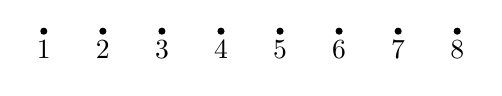
\begin{tikzpicture}[scale=0.75]
    \Matching{1}{2}\Matching{3}{5}\Matching{4}{7}\Matching{6}{8}
    \foreach \i in {1,...,8}{
      \draw [fill] (\i,0) circle [radius=0.05] ;
      \node[below] at(\i,0) {\i};
    }
  \end{tikzpicture} \qquad
  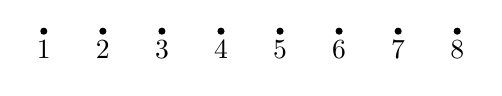
\begin{tikzpicture}[scale=0.75]
    \Matching{1}{6}\Matching{2}{3}\Matching{4}{5}\Matching{7}{8}
    \foreach \i in {1,...,8}{
      \draw [fill] (\i,0) circle [radius=0.05] ;
      \node[below] at(\i,0) {\i};
    }
  \end{tikzpicture}
  \caption{Two matchings on \( [8] \). The first one is nonnesting, while the second one is noncrossing.}
  \label{fig:matching}
\end{figure}
For an arc \( \{i,j\} \) with \( i<j \), $i$ is called an
\emph{opener} and $j$ is called a \emph{closer}. 
Let \( \Mat_{2n} \) (\( \NC_{2n} \) and \( \NN_{2n} \), respectively) stand for
the set of (noncrossing and nonnesting, respectively) matchings on \( [2n] \).

Note that there is a natural bijection between \( \SYT(n,n) \) and
\( \NN_{2n} \). For \( T\in\SYT(n,n) \), connect two vertices lying
on the same column of \( T \) via an arc, then we obtain a
nonnesting matching. For instance, the tableau in Figure~\ref{fig:SYT}
and the first matching in Figure~\ref{fig:matching} are under this correspondence.
Using this correspondence, we index the Specht basis for \( \Spec^{(n,n)} \)
by nonnesting matchings of \( [2n] \), instead of standard Young tableaux of shape
\( (n,n) \):
\[
  \{ v_M \in \Spec^{(n,n)} : M\in\NN_{2n} \}.
\]

We now consider the \( 2 \times 2n \) matrix
\[
  z = 
  \begin{bmatrix}
    z_{1,1} & z_{1,2} & \dots & z_{1,2n} \\
    z_{2,1} & z_{2,2} & \dots & z_{2,2n}
  \end{bmatrix},
\]
where \( z_{i,j} \)'s are indeterminates.
For \( 1\le i<j\le 2n \), let \( \Delta_{ij}:=\Delta_{ij}(z) \) be the maximal minor of \( z \) with respect to the \( i \)th and \( j \)th columns,
i.e., \( \Delta_{ij} = z_{1,i} z_{2,j} - z_{1,j} z_{2,i} \).
For a matching \( M\in\Mat_{2n} \), let
\[
  \Delta_M := \Delta_M(z) = \prod_{\{i,j\}\in M} \Delta_{ij} \in \CC[z_{1,1},\dots,z_{2,2n}].
\]
It is important to note that the polynomials \( \Delta_{ij} \) satisfy the following relation:
For \( 1\le a<b<c<d \le 2n\),
\begin{equation} \label{eq:syzygy}
  \Delta_{ac} \Delta_{bd}
    = \Delta_{ab} \Delta_{cd} + \Delta_{ad} \Delta_{bc}.
\end{equation}
We define a vector space \( W_n \) to be the \( \CC \)-span of \( \Delta_M \)
for all \( M\in\Mat_{2n} \).
In \cite{KR84}, it turns out that the set
\begin{equation} \label{eq:basis_NC}
  \{ \Delta_{M}\in W_n : M\in\NC_{2n} \}
\end{equation}
forms a basis for \( W_n \). We call this basis the \emph{web basis}.
(The web basis was developed in the \( \SL_2 \)-invariant theory
due to Kuperburg~\cite{Kup96},
and its original construction slightly differs from the one we describe above.
But they are essentially the same; see \cite{Rho19}.)

In addition, there is a natural \( \SYM_{2n} \)-action on \( W_n \)
as follows: Regarding a permutation \( \sigma\in\SYM_{2n} \) as
a \( 2n\times 2n \) permutation matrix, define \( \sigma\cdot \Delta_M(z)
:= \Delta_M(z\sigma^{-1}) \).
Then the space \( W_n \) is closed under this action,
and hence carries an \( \SYM_{2n} \)-module structure.
Furthermore, the \( \SYM_{2n} \)-module \( W_n \) is isomorphic to
the Specht module \( \Spec^{(n,n)} \)~\cite{PPR09}.
Therefore, due to Schur's lemma, there is a unique (up to scalar)
isomorphism \( \varphi:W_n \rightarrow \Spec^{(n,n)} \).

% We are now in a position to state our main results.
Let \( M_0 \) be the unique matching which is simultaneously noncrossing and
nonnesting, i.e., \( M_0 = \{ \{1,2\},\dots,\{2n-1,2n\} \} \).
Due to \cite{RT19}, the isomorphism \( \varphi \) maps \( \Delta_{M_0} \)
to \( v_{M_0} \) up to scalar, and thus we choose an appropriate scalar so that
\( \varphi(\Delta_{M_0}) = v_{M_0} \).
We also let \( w_M := \varphi(\Delta_M) \) for each \( M\in\NC_{2n} \).
Then the Specht basis can expand into (the image of) the web basis:
For \( M\in\NN_{2n} \),
\[
  v_M = \sum_{M'\in\NC_{2n}} a_{MM'} w_{M'}.
\]
In \cite{RT19}, Russell and Tymoczko initiated the combinatorial study of
the transition matrix
\[
  A = (a_{MM'})_{M\in\NN_{2n}, M'\in\NC_{2n}}.
\]
They constructed directed graphs on the standard
Young tableaux and noncrossing matchings, and using them,
showed the unitriangularity of the matrix.
They also gave some open problems related to their results.
One of them is the positivity of the entries of \( A \),
which was proved by Rhoades soon after.
\begin{thm}[\cite{Rho19}]
  The entries \( a_{MM'} \) of the transition matrix \( A \) are
  nonnegative integers.
\end{thm}
Although Rhoades established the positivity phenomenon for entries of \( A \),
he did not find an explicit combinatorial interpretation of the nonnegative integer \( a_{MM'} \), c.f. \cite[Problem 1.3]{Rho19}.
Inspired by his work, we introduce a new family of permutations which
are enumerated by the integers \( a_{MM'} \), and study their enumerative
properties.

Our strategy is based on Rhoades's observation~\cite{Rho19}.
He figured out that the entries \( a_{MM'} \) are related to resolving crossings
of matchings in the following sense:
For a matching \( M\in\Mat_{2n} \), let \( \{ a,c \} \) and \( \{ b,d \} \) be
a crossing pair in \( M \) (if it exists) where \( a<b<c<d \).
Let \( M' \) and \( M'' \) be the matchings identical to \( M \) except that
\( \{ a,b \} \) and \( \{ c,d \} \) in \( M' \), and
\( \{ a,d \} \) and \( \{ b,c \} \) in \( M'' \).
Then, by the relation \eqref{eq:syzygy}, we have
\begin{equation}\label{Eq: web relation}
  \Delta_M = \Delta_{M'} + \Delta_{M''}.
\end{equation}
In addition, the number of crossing pairs in \( M' \) (respectively, \( M'' \)) is
strictly less than the number of crossing pairs in \( M \).
Therefore, iterating the resolving procedure gives the expansion of \( \Delta_M \)
in terms of the basis \eqref{eq:basis_NC}.
In other words, when we write 
\begin{equation} \label{eq: web expansion}
  \Delta_M = \sum_{M'\in\NC_{2n}}c_{MM'} \Delta_{M'},
\end{equation}
the coefficient \( c_{MM'} \) is equal to
the number of occurrences of the noncrossing matching \( M' \)
obtained by iteratively resolving crossings in \( M \).
Note that the order of the choice of crossing pairs does not affect the expansion of \( \Delta_M \).
Rhoades showed that for \( M\in\NN_{2n} \) and \( M'\in\NC_{2n} \),
the entry \( a_{MM'} \) of the transition matrix equals \( c_{MM'} \).
Hence, to give a combinatorial interpretation of \( a_{MM'} \), we track
the resolving process from a nonnesting matching to noncrossing matchings.

To state our main result, we need some preliminaries.
We first note that noncrossing matchings and nonnesting matchings are \emph{Catalan objects}.
In other words, they are enumerated by Catalan numbers.
Another famous Catalan object is a Dyck path.
A \emph{Dyck path} of length \( 2n \)  is a lattice path from \( (0,0) \)
to \( (n,n) \) consisting of \( n \) north steps \( (0,1) \) and
\( n \) east steps \( (1,0) \) that does not pass below the line \( y=x \).
We write \( \NS \) and \( \ES \) for the north step and the east step,
respectively.
We therefore regard a Dyck path as a sequence consisting of
\( n \) \( \NS \)'s and \( n \) \( \ES \)'s.
Let \( \Dyck_{2n} \) be the set of Dyck paths of length \( 2n \).
Identifying a Dyck path with the region below the path,
we give a natural partial order on \( \Dyck_{2n} \) by inclusion,
denoted by \( \subseteq \).
For instance, the Dyck path \( \NS\cdots\NS\ES\cdots\ES \) where
\( n \) \( \NS \)'s precede \( n \) \( \ES \)'s is the maximum path
in \( \Dyck_{2n} \) with respect to the partial order,
while the path \( \NS\ES\NS\ES\cdots\NS\ES \) is the minimum path.
In Section~\ref{sec:grid configuration}, we define a map
\( D:\Mat_{2n}\rightarrow \Dyck_{2n} \), and by abuse of notation,
a map \( D:\SYM_n\rightarrow \Dyck_{2n} \).
We also define a map \( M:\SYM_n\rightarrow \NC_{2n} \).
Finally, we introduce a new family of permutations,
called \emph{web permutations}. With these data, we now present one of our main
results.
\begin{thm} \label{thm:main_intro}
  For matchings \( M\in\NN_{2n} \) and \( M'\in\NC_{2n} \),
  the entry \( a_{MM'} \) is equal to the number of web permutations
  \( \sigma\in\SYM_n \) such that \( D(\sigma)\subseteq D(M) \) and \(M(\sigma)=M'\).
\end{thm}

The theorem follows almost immediately from the definition of the novel
permutations.
However, the definition does not directly tell us whether a given permutation
is a web permutation or not.
Our second main result, Theorem~\ref{thm:web=andre_cycle}, 
explains how to characterize these permutations in terms of their cycle structures.
Using this characterization, we deduce the results in \cite{RT19,IZ22}
concerning the unitriangularity of the transition matrix and a necessary
and sufficient condition for additional vanishing entries.
Furthermore, the characterization leads us to enumerative properties of web
permutations.
To be more precise, Euler numbers count web permutations (Corollary~\ref{cor:Euler}), and we present
a conjecture related web permutations and the Seidel triangle, which generalizes
a result of Nakamigawa~\cite{Nak20} (Conjecture~\ref{conj:Seidel}).

The article is organized as follows.
In Section~\ref{sec:grid configuration}, we give a new model,
called a grid configuration, for representing matchings.
Within this model, we resolve crossings in nonnesting matchings
until there is no crossing.
We then define web permutations from the noncrossing grid configurations,
and prove Theorem~\ref{thm:main_intro}.
In the next two sections, we study some properties of web permutations.
In Section~\ref{sec:characterization}, we give a characterization of
web permutations. We show that web permutations are closely related to
Andr\'e permutations.
Section~\ref{sec:enumeration} provides some interesting enumerative properties
of web permutations.
% For example, web permutations are enumerated by Euler numbers.
% We also give a conjecture for a relation between certain web permutations
% and the Seidel triangle.